% Do not change the options here
\documentclass[bsc,frontabs,parskip,deptreport]{infthesis}

\usepackage{graphicx}
\usepackage[%  
    colorlinks=true,
    pdfborder={0 0 0},
    linkcolor=black,
    citecolor=blue
]{hyperref}
\usepackage[authoryear,comma]{natbib}
\usepackage{csvsimple}
\usepackage{fancyvrb}
% \setcitestyle{authoryear,comma,open={(},close={)}} 

\newcommand{\coderepo}{\href{https://github.com/LasseWolter/laughter-detection-icsi}{github-repo} }

\begin{document}
\begin{preliminary}
\title{A Zoom filter for applause and laughter}

\author{Lasse Wolter}

% to choose your course
% please un-comment just one of the following
%\course{Artificial Intelligence}
\course{Artificial Intelligence and Computer Science}
%\course{Artificial Intelligence and Mathematics}
%\course{Artificial Intelligence and Software Engineering}
%\course{Artificial Intelligence with Management}
%\course{Cognitive Science}
%\course{Computer Science}
%\course{Computer Science and Management Science}
%\course{Computer Science and Mathematics}
%\course{Computer Science and Physics}
%\course{Computer Science with Management}
%\course{Software Engineering}
%\course{Software Engineering with Management}

\project{4th Year Project Report}

\date{\today}

\abstract{

% This skeleton demonstrates how to use the \texttt{infthesis} style for
% undergraduate dissertations in the School of Informatics. It also emphasises the
% page limit, and that you must not deviate from the required style.
% The file \texttt{skeleton.tex} generates this document and can be used as a
% starting point for your thesis. The abstract should summarise your report and
% fit in the space on the first page.
}

\maketitle

\section*{Acknowledgements}


\tableofcontents
\end{preliminary}


% The preliminary material of your report should contain:
% \begin{itemize}
% \item
% The title page.
% \item
% An abstract page.
% \item
% Optionally an acknowledgements page.
% \item
% The table of contents.
% \end{itemize}

\chapter{Introduction}

Achievements
\begin{enumerate}
  \item Evaluation of existing laughter detection model on the whole ICSI meeting corpus
  \item Investigation of bad performance of this model on ICSI corpus
  \item Retrain model on ICSI corpus
\end{enumerate}

\chapter{Background} \label{cha:bg}
Automatic applause and laughter detection isn't a new idea. Nevertheless, the research in these two areas is usually done separately. There are a few papers which cover both, one of the most popular ones being from Cai et al. \citep{cai2003highlight} who used sound effect detection - which included laughter and applause - for video summarisation and highlight extraction.
Apart from this and a few other papers most research only covers one of the two domains, either applause or laughter. Thus, we split the review of existing research into the following sections:
\begin{enumerate}
  \item Laughter Detection
  \item Applause Detection
  \item Evaluation Metrics 
\end{enumerate}


\section{Laughter Detection} \label{sec:bg-laughter}
The investigation of the acoustic features of laughter reaches back three decades \citep{bickley1992acoustic}.
In the early 2000s, the first attempts of laughter detection in conversational speech classified presegmented audio data \citep{kennedy2004laughter, truong2005automatic}. These models could only decide whether laughter occurred within in a given segment. The determination of segment boundaries of laughter events wasn't considered. 
Corpora used in these papers include the development data from the 2004 Spring NIST Rich Transcription Evaluation \citep{ldcnistcorpus}, the Dutch CGN corpus \citep{oostdijk2000spoken} as well as the ICSI Meeting Recorder corpus \citep{morgan2001meeting}. 

Two examples of such classification of presegmented audio data were presented by Kenney and Ellis \citep{kennedy2004laughter} and Truong and Van Leeuwen \citep{truong2005automatic}. 
Even though both models classified presegmented audio there were some significant differences. 
Firstly, the definition of laughter and the motivation behind the research differed.
While Kennedy and Ellis define laughter events as 'points in the meeting where more than one person laughs', Truong and Van Leeuwen considered one person laughing as a laughter event.
Kennedy and Ellis did not specify a particular motivation whereas Truong and Van Leeuwen's long-term goal was the investigation of 'paralinguistic events' - laughter being one of them - to classify the speaker's emotional state.   

Secondly, there was a difference between the best performing features and predictors.  
Kennedy and Ellis \citep{kennedy2004laughter} got the best results using Mel Frequency Cepstral Coefficients (MFCCs) as features and a Support Vector Machine (SVM) for decision making. 
In contrast, Truong and Van Leeuwen \citep{truong2005automatic} used Perceptual Linear Prediction (PLP) features with Gaussian Mixture Models (GMM) for classification. 

Truong and Leeuwen \citep{truong2007automatic} continued their research and stated that spectral features alone (such as PLP and MFCCs) can be used to discriminate between laughter and speech but a significant improvement can be achieved when using prosodic features - features relating rhythm and intonation.

In 2006, Knox and Mirghafori \citep{knox2006automatic} were the first to do laughter recognition without the need for presegmented audio data.  
They worked with the Bmr-subset of the ICSI Meeting corpus \citep{morgan2001meeting} to be able to compare their results to previous research done on this dataset \citep{kennedy2004laughter, truong2005automatic, truong2007automatic}.

Their goal was to obtain accurate interval boundaries of laughter segments.
One limiting factor for the precision of these boundaries is the frame size. 
When Knox and Mirghafori first experimented with SVMs similar to Kennedy and Ellis \citep{kennedy2004laughter}, they realised that the time to compute the features and train the SVM increased significantly with decreasing frame size. 
This is because aggregate statistics need to be calculated and stored for each frame of training data.  
On the contrary, a neural network trained with features from a context window can directly use the features of each frame without aggregating them.  

To obtain frame-level training labels for the ICSI dataset Knox and Mirghafori first removed all segments that contained both speech and laughter under a single start and end time because the laughter specific interval boundaries couldn't be identified in those segments. 
The remaining audio data could be accurately separated into laughter and non-laughter segments which were then divided into 10ms frames and labeled accordingly.

The model was trained to classify each 10ms frame using a window of 75 frames around the target frame - 37 before and 37 after the frame (\ref{fig:know_window}).
This way an accurate prediction of laughter boundaries of up to 10ms was possible. 
The features investigated by Knox and Mirghafori are MFCCs, AC PEAK, F0 and RMS as well as their corresponding delta and delta-delta features.
They first trained four separate neural networks each one taking one of the mentioned features as input.
Afterwards they combined the different models by using their output as input for another, smaller neural network.
The best results were obtained by combining the outputs of three NN-systems which used delta MFCCs, AC PEAK and F0 as features, respectively.
By training and evaluating separate neural networks for each type of feature first, Knox and Mirghafori observed that MFCCs have the most discriminative power which aligns with prior research by Kennedy and Ellis \citep{kennedy2004laughter}.

\begin{figure}[htp]
    \centering
    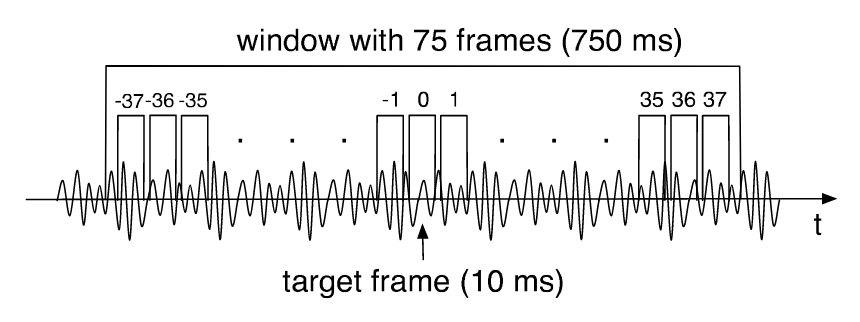
\includegraphics[width=10cm]{imgs/Knox_window.png}
    \caption{Frame window used by Knox and Mirghafori}
    \label{fig:know_window}
\end{figure}

A survey from 2016 \citep{cosentino2016quantitative} investigates research on laughter and laughter detection in different fields up to that time.
This survey covers different detection methods using visual, acoustic and sensory data.
For this thesis laughter detection using solely acoustic features is the most relevant. Consentino et al. \citep{cosentino2016quantitative} find that in such cases best performance was obtained using MFCCs and PLPs as features and combining the resulting classifier with ones that also use prosodic features.
This aligns with findings from prior research \citep{truong2007automatic, knox2006automatic}.

More recent research by Gillick et al. \citep{gillick2021robust} finds that features learned from spectrograms using deep convolutional networks outperform previous approaches based on MFCCs.
Their hypothesis was that models using MFCCs are more prone to pick up surface level characteristics of sound and thus, will be more sensitive to variations like background noise.
Gillick et al. expected that features learned using a CNN are more representative of the actual laughter and thus, more robust to different environments. 
Their results show that a model using features learned by a CNN architecture outperforms the conventional approach using MFCCs. 


\section{Applause}
The following review is less exhaustive because we decided to focus on laughter detection for now. Applause detection is a possible extension of the project. 
More information on this decision can be found (TODO: Link to corresponding section).

As mentioned at the beginning of this chapter, in 2003 Cai et al. \citep{cai2003highlight} worked on the detection of sound events, including applause.
They used perceptual features and MFFCs as features, Hidden Markov Models (HMM) and Gaussian Mixture models (GMM) to model sound and log likelihood for decision making.
Cai et al. evaluated their system on a testing set consisting of 2 hours of video material from different programs.
For applause specifically they achieved a precision of 87.37\% and a recall of 92.00\%.

In contrast, Uhle \citep{uhle2011applause} used MFCCs and low-level descriptors (LLD) to represent sound and passed these features to an MLP or an SVM for classification.
The difference between MLP and SVM classifier were rather small.
Uhle worked with a relatively small dataset consisting of 210 segments of 9-30s length. This equates to a total length between 31.5 min and 105 min.
On a rather small test (10\% of this dataset) Uhle achieved an accuracy of 95\% with a precision 96.51\% and recall of 97.65\%.

A less complex approach for applause detection was presented by Li et al. \citep{li2009characteristics}.
They used a manually created 4-layer decision tree to classify a given sound input as applause or not-applause.
Testing their model on 50 hours of meeting speech containing 500 applause segments ranging from 0.8 to 36s they were able to retrieve 491 of the 500 applause segments while incorrectly retrieving 38 non-applause segments.
This equates to a recall of 98.2\% and a precision of 92.82\%. Li et al. also compared their less complex model to the HMM model proposed by Cai et al.\citep{cai2003highlight} and outperformed it while using less computational time.

Manoj et al. \citep{manoj2011novel} proposed another approach based on manually created decision trees. They also compared it to a more complex model similar to the one proposed by Cai et al. \citep{cai2003highlight} - with the difference that this model only used GMMs, no HMMs.
Even though the decision tree stages were different to Li et al. \citep{li2009characteristics} the findings are similar. The decision tree outperforms the more complex method using MFCCs and GMMs.  

\section{Evaluation metrics} \label{theory}
\subsection{Accuracy, Precision and Recall} \label{sec:acc-prec-rec}
Accuracy, precision and recall are standard metrics for performance evaluation.
All three metrics are calculated by comparing the predicted class lables to the true class lables.
Without going into much detail this section states the formulae, their meaning for our use case and advantages of one metric over the other.
Let:
\begin{enumerate}
    \item $TP$: True Positives - laughter samples correctly classified as laughter
    \item $FP$: False Positives - non-laughter samples incorrectly classified as laughter
    \item $TN$: True Negatives - non-laughter samples correctly classified as non-laughter
    \item $FN$: False Negatives - laughter samples incorrectly classified as non-laughter
\end{enumerate}
\textbf{Accuracy}: Percentage of correctly classified samples (laughter and non-laughter) over the total number of samples.
$$Accuracy = \frac{TP+TN}{TP+TN+FP+FN}$$
\textbf{Precision}: Percentage of correctly classified laughter samples over all samples predicted as laughter.
$$Precision = \frac{TP}{TP+FP}$$
\textbf{Precision}: Percentage of correctly classified laughter samples over all laughter-samples.
$$Recall = \frac{TP}{TP+FN}$$

\subsection{Binary Cross Entropy Loss}
In comparison to accuracy, precision and recall (\ref{sec:acc-prec-rec}) the loss of a model is computed from the raw probabilities output by the model, not the predicted labels which are inferred from this probability.

A the model of our binary classifier outputs a probability between 0 and 1. Only applying a threshold turns this probability into a class label. This threshold is a variable parameter.
For example, with a threshold of 0.5 all predicted probabilities of 0.5 and higher are output as class 1, in our case laughter. All probabilities below 0.5 are output as non-laughter. 
Varying this threshold changes the predicted labels and thus, yields different performance in terms of precision and recall. 

In contrast, the loss of a model's output is independent of the threshold as it is calculated directly from the probabilities.
When a machine learning algorithm learns how improve its predictions it minimises this loss. There are different functions for calculating loss.
A typical approach for classification problems is the Cross Entropy Loss. Since our use case only has two classes (laughter and non-laughter) we can use Binary Cross Entropy Loss. 

Assume we have a two vectors $P$ and $Y$ of length $m$. For each of the $m$ samples $P$ contains the probability of the sample being laughter whereas $Y$ contains its true class (laughter $\Rightarrow y=1$, non-laughter $ \Rightarrow y=0$).
Given this, the model's Binary Cross Entropy Loss is given by:
$$ L(P,Y) = \sum_{n=1}^{m}  -{(y*\log(p) + (1 - y)*\log(1 - p))}$$

To understand the meaning of this equation we look at a single sample with predicted probability \texttt{p} and a true class value of \texttt{y}. Its Binary Entropy Loss is given by: 
$$ L(p,y) = -{(y*\log(p) + (1 - y)*\log(1 - p))} $$
We know that one of the terms $y$ and $(1-y)$ will always be zero.
Thus, we are left with the negative log of the probability that the sample belongs to the true class, e.g. a sample with $p=0.8$ is predicted to be laughter with an 80\% chance and non-laughter with a 20\% chance. Negative log ensures that $L(x,y) > 1  \forall x $. 
Due to the logarithmic nature of this loss-function confidently misclassified examples (e.g. $p=0.1$) are punished more heavily than unconfidently misclassified examples (e.g. $p=0.4$).

To summarise, the Binary Cross Entropy Loss captures how far off the predictions of the model are from the true values. It sums negative log probabilities of belonging to the true class and punishes confidently misclassified samples more heavily.

\subsection{Confusion Matrix}
TODO
special case - because it's only a 'one-sided' confusion matrix.

\chapter{tbd} 

\section{Model and data selection}\label{sec:model-and-data}
After having done the initial research we decided to focus solely on laughter detection. 
There are two main reasons for this, type of previous research and open source code available.  
As mentioned in the background chapter (\ref{cha:bg}) most research in the field of laughter and applause detection is done separately. 
Thus, implementing a detection algorithm from existing research requires merging different models. 
For a combined model to work a good understanding of each domain is essential.
We decided that this is most easily attained by focusing on one domain first. 
We chose to focus on laughter instead of applause because there was an open-source repository available which showcased an existing state-of-the-art laughter detection algorithm \citep{gillick-codebase}.
In fact, the corresponding paper by Gillick et al. \citep{gillick2021robust} was just published a month before this project started.

The domain we are working with in video conferences is separate single person audio tracks usually recorded in a relatively quiet environment.
To investigate how the existing model might perform in this domain, we decided to evaluate it on the ICSI meeting corpus \citep{morgan2001meeting}. 
We initially considered the use of Audio Set \citep{googleaudioset} as a possible evaluation corpus. After some discussion we discarded this idea because of a mismatch with the domain for our project. Audio Set  consists of 10s audio segments from Youtube videos which were labeled according to a fixed set of classes - including laughter. Nevertheless, the domain of Youtube videos varies drastically. It can be a recording of someone laughing in a silent environment inside a room or someone laughing in a very noisy environment outside. This variety of environments might help for generalising laughter detection but isn't suitable for our project.
In contrast, the ICSI corpus was a good match to our domain as it solely consists of meeting speech recorded with both close-distance and table-top microphones. 
We only make use of the close-distance microphone recordings which capture the audio of a single meeting participant.
Laughter occurrences aren't reported by class assignment as in Audio Set. The ICSI corpus provides transcriptions for all its participants containing speech as well as \texttt{Vocal} and \texttt{NonVocal} tags for sounds like microphone noise and laughter. 
Another reason for choosing the ICSI corpus is it is size - about 72 hours.
Even after filtering for laughter segments that occur on their own, there are still 8420 segments with an accumulated duration of 3.9h. 
We considered this a reasonable size to do evaluation on. 




\section{Model Evaluation} \label{sec:model-eval}

\subsection{Filter out laughter only segments} \label{subsec:filter-laughter}
ICSI transcriptions are split into segments denoted by a start and end time.
Consequently laughter segments co-occurring to speech in one segment cannot be precisely identified.
Such laughter transcriptions are also called weakly labeled. Weakly labeled means that only the presence or absence of an event is given, whereas strongly labeled data states precise boundaries.
Strongly labeled data is key for this project.
Filtering for strongly labeled laughter segments resembles Knox and Mirghafori's approach to obtain frame-level training data \citep{knox2006automatic} (\ref{sec:bg-laughter}). 
After applying this approach I ended up with TODO laughter segments.

Alternatively, I could have created an ASR model to align weakly-labeled laughter events with their audio counterpart. 
I did not follow this approach for two reasons: it would have more time consuming and the amount of data achieved with the above approach was sufficient. 
Future projects might consider this approach to gain strongly labeled data for the whole corpus. 

\subsection{First evaluation}
In contrast to some existing research \citep{kennedy2004laughter, knox2006automatic} which only used a subset of the ICSI corpus we used the whole dataset for evaluation. We ran the pre-trained detection model by Gillick et al. with four different thresholds for each channel of the 75 meetings - a total of 468 audio tracks. 
Precision and recall for those 1872 experiments can be found in table (TODO).
A precision-recall curve was plotted (fig:TODO). The precision recall curve has the expected shape but visualises the main problem. The maximum recall achieved is 31.53\%. We expected that a low threshold like 0.2 would yield low precision. Getting such a low recall, however, was surprising. 
Initially we thought that there might be something wrong with our evaluation method. After some discussion we realised that the discarded laughter occurrences to get strongly labeled data weren't discarded from the predictions. This meant that the model could classify a laughter occurrence correctly but the evaluation method would consider it as false because this laughter occurrence was discarded pre-evaluation. This discrepancy in preprocessing was easily fixed and improved the precision significantly (fig: TODO). Nevertheless, the recall remained almost unchanged. 

To make these results more tangible we did a theoretical experiment. What would happen is such is system was deployed? The results of this practical experiment can be seen in table TODO. 
Considering any of the four possible systems - with different thresholds each - it is aparent that such a system would be entirely unusable. We'll briefly examine the two extreme cases. If the threshold was really low, e.g. 0.2, not roughly TODO minutes of TODO minutes laughter would be correctly retrieved. Despite this being a not even half of the laughter events that actually occurred we also got about TODO minutes of noise.  
On the other hand, choosing a high threshold, e.g. 0.8, yields very high precision and thus, no noise is transmitted. Even though no noise is retrieved we merely retrieve TODO minutes of laughter in a meeting of TODO minutes. With such a low percentage of retrieved laughter events there is not much difference to entirely muting yourself. 

A possible reason for such a bad performance on the ICSI corpus is a data mismatch between training and evaluation data. The pre-trained model by Gillick et al. \citep{gillick2021robust} was trained on the Switchboard corpus \citep{switchboard-corpus}. The Switchboard corpus records telephone conversations between two participants at a sample rate of 8000hz. The ICSI corpus records meeting speech of multiple participants at a sample rate of 16000hz. The Switchboard dataset has one audio track containing all audio whereas the ICSI corpus has a separate audio track for each participant.  
TODO: possible other differences?
These differences suggest that a model trained on one of these corpora might not perform well on the other one. 
TODO: How does this tie in with Gillick et al.'s statement that they tried to create a detection algorithm that performs better on noisy data? How do they define "work well"? Did this cause the model to perform worse on quiet data?
In response to this finding we decided to retrain the model on the ICSI dataset. 

\chapter{tbd}
\section{Retraining the model} \label{sec:retraining}
The first approach was to adapt the code that Gillick et al. used and published \citep{gillick-codebase}. After investigating their code, I created a diagram of their data-pipeline (TODO: add figure). 
I created a similar one for our project and after consultation with my supervisors decided that the hash-map containing the preloaded audio could be neglected for now. 

After looking at the code in more detail, I realised that it was cumbersome and disregarded current standards of pytorch programs. 
For example, they used a manual batch counter for training steps instead of using epochs.  
Design decisions like this make the code harder to read and harder to debug. 
Gillick et al. programmed lots of augmentation and transformation functions themselves instead of using existing implementations from libraries like pytorchaudio [TODO add link]. 
Programming functions for turning audio files into spectrograms and padding/truncating audio files to a certain length themselves, makes the code unnecessary long and introduces risk for errors. In my opinion using existing and exhaustively tested functions from a popular framework like pytorchaudio is better in terms of readability, efficiency and stability of the code.
My supervisor doesn't have much experience with pytorch but agreed that he doesn't consider the code as well written.

Despite the concerns about Gillick et al.'s code mentioned above, I decided to try to adapt their code for two main reasons. 
Firstly, I haven't worked on an ML project of this scale before and writing training and inference code from scratch seemed somewhat daunting to me. Further, I trusted that the code that Gillick et al. published should be usable as they have used it for a paper they published \citep{gillick2021robust}. 
Secondly, I thought that using their code and just doing minimal adjustments would allow for an easier comparison between the two data sets. If I wrote the code from scratch I'd have to make sure that all the preprocessing and model parameters are sufficiently similar to state the difference of changing the training data. 

After adapting the training code for about a week I ran into a major problem. Training the model was really slow. The model trained around 30 batches of audio in two hours, each consisting of 32 audio tracks. 
With training samples of 1 second each this equates to one sample every eight seconds.
This training performance on a GPU machine is significantly slower than the evaluation on a CPU-only machine. TODO:cite rtf table

After some further investigation I realised that the data-loading is the bottleneck. I ran some experiments to check how long it takes to load the data (TODO: add exp data) and found that it's unacceptably slow. 
I also investigated the librosa loading times from different offsets in an audio file. It turned out that the loading time of a sample of an audio track grows linearly with the offset at which this sample is located. [TODO: add graph/table]

I discussed these results with my second supervisor and he suggested that it might be due to the different recording length of the switchboard dataset. According to LDC data \citep{switchboard-ldc} the switchboard dataset contains 2400 recordings and a total of approximately 260 hours of speech. This equals an average recording length of roughly 6.5 minutes. Compared to around 58 minutes average \citep{icsi-ldc} of the ICSI recording corpus this is a significant difference.


As mentioned before I hadn't done the preloading of audio data like Gillick et al.. 
I thought about adding that to the pipeline but realised that it doesn't work because the accumulated data won't fit into memory. 
The following estimates show the difference in storage space needed to preload the whole ICSI/Switchboard corpus as .wav-files. We assume a bitrate of 16bits = 2bytes per sample.

Gillick et al. were able to fit all audio data into memory because all switchboard recordings consist of only one audio file which contains the recordings from both participants. Thus, we have 260 hours of raw audio sampled at 8khz which can be estimated as:

\[ \frac{260hours * 3600 seconds * 8000 samples per second * 2 bytes}{1024^3} \approx 13.95 GB \]

For the ICSI corpus we are using the close-microphone recordings which record each speaker individually. Thus, with an average participant number of 6 we have 72*6=432 hours of audio sampled at 16khz:

\[ \frac{432 hours * 3600 seconds * 16000 samples per seconds * 2bytes}{1024^3} \approx 46.35 GB \]

This shows that using a machine with lots of RAM would allow loading the whole audio data into memory. 
Regardless of my missing access to such a machine I considered this bad practice and decided to rewrite the dataloader from scratch. 

My second supervisor suggested looking at Lhotse \citep{zelasko2021lhotse} a new python library for speech and audio data preperation. It's still in development but at a state where it's already usable.

\subsection{Lhotse}
Two main feature that make Lhotse suitable for my use case are:
\begin{enumerate}
    \item Simplified loading of popular corpora like ICSI
    \item Sample creation without actually loading audio data from disk
\end{enumerate}

Lhotse provides so called \textit{recipes} which simplify working with popular corpora like the ICSI corpus.
These \textit{recipes} are python scripts that create \textit{manifests}.
\textit{Manifests} are representation of the entire corpus which contain only meta data of the recordings as well as the corresponding supervisions. 
Only by using this metadata Lhotse can create samples - Lhotse calls them \textit{Cuts} - without loading any audio or transcript data into memory. 

Due to Lhotse being in development I needed to make some adjustments myself. The recipe for the ICSI corpus wasn't part of the latest release \textit{v0.12} which meant that I had to work with the development version. I fixed some bugs in the ICSI recipe to make it work. I also ran into some other issues with Lhotse and decided to debug some of them. Some of the debugging wasn't strictly necessary for my project. Nevertheless, I decided to spent the time on this because I wanted to contribute to this open source project which has potential to be useful in the field of audio and speech processing in the future (list contributions?).
Contributions: 
\begin{itemize}
    \item improved/debugged ICSI recipe 
    \item bug when trying to compute features with multiple workers in parallel (TODO: add link?).
\end{itemize}

For this project, I did not make use of the supervisions in the manifest but created them manually for each segment. (TODO: add example of supervision segment)
The reason for this is that I already had an existing dataframe with laughter and speech segments and a code that generates variants of such dataframes.
The generated dataframe contained all information needed for a supervision segment, the channel, the start and end time of a segment as well as its label. 
I used the label in each row in the dataframe to create a custom supervision segment stating if this segment was laughter or not. 
This way I could simply adapt a voice activity detector dataset already provided by Lhotse(TODO Link). Due to the preprocessing applied, all segment in the dataframe are either fully laughter or no laughter at all.
Thus, the data is strongly labeled even though the lables are binary.
For future use and trying alternative audio segmentation - e.g. segments containing laughter and speech - it would be better to compute the supervision segments from the original manifest.  


The feature representation is another important design decision. Gillick et al. \citep{gillick2021robust} used a Melspectrogram, representing each second of audio with a 44 by 128 feature matrix. 44 means 44 samples per 1 second. 128 means that each sample is represented by 128 values, i.e. 128 mel-bins. They don't state explicitly why they have chosen this shape. 
Experimenting with different shapes is important to investigate its impact on the real-time-factor and performance.  

\chapter{ML Pipeline}



\chapter{Experiments} \label{cha:experiments}

\section{Experiment 1}

\section{Experiment 2a} \label{exp:2}
This set of experiments evaluates the effect of the structure of training data on the final model performance. Structure here refers to two things: 
\begin{enumerate}
    \item class balance between laughter and non-laughter samples
    \item diversity of non-laughter samples 
\end{enumerate}


The second factor is class diversity. Even though laughter detection is a binary classification problem there are lots of types of non-laughter, the most obvious distinction being speech and silence. Having a good representation of this diversity of non-laughter segments is essential for a good performance of the model.
In our evaluation we distinguish five different kinds of non-laughter:
speech, silence, vocal-sounds, non-vocal-sounds, invalid segments. 

\subsection{Method}
\subsubsection{Experiment 2A}
In the first set of experiments different ratios between laughter and non-laughter segments in the training data were evaluated. 
The non-laughter segments were selected on a random basis from remaining audio tracks after subtracting the laughter and invalid regions (see types of segments - TODO add ref). 
Three different ratios were tried where the amount of non-laughter segments was gradually increased from the same amount, over 10 times as many, to 20 times as many non-laughter segments.
All samples were one second long and there was no subsampling applied during training.

To select non-laughter segments across a variety of meetings the following selection process was used.
For each laughter segment a non-laughter segment of the same duration was sampled from the same meeting. It is possible that the sample if from a different speaker, the channel within that meeting is chosen at random.
If the laughter segment was longer than one second, both laughter and non-laughter segments were truncated to a random one second region of their segment. 
If the segment was shorter than one second, it was stored as is and padded during feature computation.
All these segments were stored in a table as shown in \ref{table:data-df}.
The code creating this table can be found in \verb|create_data_df.py|. 

For each segment in this table an Fbank feature representation of shape 100x40 was created (\ref{fig:fbank-sample}). 100 stands for 100 samples, each of length 10ms. 40 stands for the number of Fbank-filters. These dimensions were chosen as they are a standard in the ASR community.
The \texttt{demo-notebook} on google collab linked from the \coderepo shows a simplified version of how \verb|compute_features.py| computes features. 
The main difference is that the provided example loads the audio file directly into a Lhotse Cut whereas \verb|compute_features.py| loads already computed feature representation of the whole meeting and only selects a the requested subset. In practice this is a lot faster for computing large amounts of features.

\subsubsection{Experiment 2B}
The second set of experiments investigated the impact of more balanced non-laughter segments. The general selection and feature computation process was similar. The only difference is that non-laughter segments weren't chosen at random but a fixed percentage of non-laughter segments was assigned to the three types of non-laughter - speech, noise and silence.
The ratio between laughter and non-laughter segments was set to 1-to-20 for all these experiments. The reason for this is that a larger amount of non-laughter segments seemed more promising to allow conclusions about its structure. 
Different percentages were tried to evaluate this impact.

\section{Experiment 3}
The reason for running this experiment is that the first few models I trained on the ICSI corpus had the same performance on both training and development set.
Usually you shouldn't evaluate on the training set because the ML model already knows that data. That's why I surprised me that the performance was so poor. So I decided to investigate this further with another set of experiments.

\subsection{Method}
Choose one meeting from the training set - 

TODO: Show initial evaluation on dev vs train set
TODO: Overfit one meeting completely and hopefully get high performance on the meeting to proof that the model works.

\begin{figure}[htp]
    \centering
    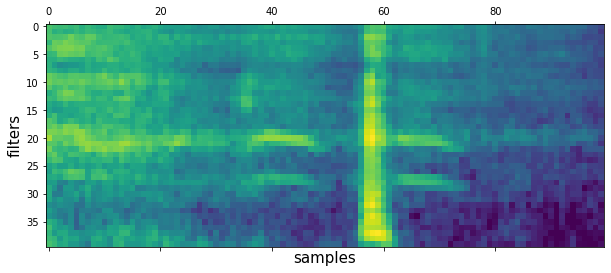
\includegraphics[width=14cm]{imgs/sample_fbank_feat.png}
    \caption{Example feature representation of a 1s laughter segment}
    \label{fig:fbank-sample}
\end{figure}


\label{table:data-df}
% \csvautotabular{csvs/data_dfs/tiny_sample.csv}

then we selected 10 and 20 times as many speech segments as laughter segments (1-to-10 and 1-to-20). 
Looking at the results.


\csvautotabular{csvs/1_to_10/dev_eval.csv}

% \begin{document}
%     \begin{tabular}{l|c}%
%     \bfseries Person & \bfseries Matr.~No.% specify table head
%     \csvreader[head to column names]{dev_eval.csv}{}% use head of csv as column names
%     {\\\hline\givenname\ \name & \matriculation}% specify your coloumns here
%     \end{tabular}
% \end{document}

\textbf{General ML advice}
When using online validation, the number of validation batches matters a lot. To get a better intutition about this I plotted the metrics during training for different batch sizes and log frequency


Another issue I ran into was that that the precision for threshold 1 wasn't 100\% and the recall for threshold 0 wasn't 100\% either. After some debugging I found a bug in Gillick et al.'s model. 
The model sometimes yields probabilities smaller than 0 and larger than 1. The overhead was usually smaller than 0.02. I did not spent time on finding the exact reason for this bug but capped the output 0 and 1, respectively.
This happens when evaluating the original model and newly trained ones.

\chapter{Lessons Learned}

\section{Use of published code}
In hindsight, I would be more careful in choosing the codebase I base my work on.
Working with sparsely documented code that doesn't adhere to certain standards (e.g. for pytorch training) slowed down my working progress. 
Missing experience in the field and the paper's publication at Interspeech 2021 made me think that it was a good codebase to work with.
Only during retraining the model and working more closely with the codebase I realised certain bugs and issues with the original code, including:
\begin{enumerate}
    \item unnecessary long training code (\ref{sec:retraining})
    \item lots of unused function
    \item a bug that the model outputs probabilities out of bounds ($<0$ or $>1$) (\ref{sec:experiments})
    \item sub-optimal code like recreation of a large object inside a for-loop even though it's independent of it
    \item mistakes in use of python operators like slicing - e.g. using \texttt{min} \texttt{np.min(probs[i:i+1])} even though this only returns 1 probability - end index is non-inclusive
\end{enumerate}

\chapter{Other}

The computations for ML training and evaluation were run on a slurm cluster of the university \citep{yoo2003slurm, tange2011gnu}.

The 72 meetings were split into training, development and test set to minimise speaker overlap. The partitioning follows the structure from \citeauthor{renals2014neural}. It uses meetings \texttt{(Bmr021, Bns001)} as development set and meetings \texttt{(Bmr013, Bmr018, Bmr021)} as test set.


\section{Practicality}
In this section I will talk about the practicality of a laughter recognition feature integrated in a video-call system. 
This section is split into two parts: 
\begin{enumerate}
    \item General practicality of such a system
    \item Alternative solutions to using a machine learning approach 
\end{enumerate}

\subsection{General practicality} \label{sec:general-pract}
Even though users will be able to opt out of using this feature, it is important to think about privacy. If most users do not feel comfortable using such a system, it will significantly affect its practicality.  
The audio of every meeting participant will be constantly analysed. Even if the system promised to discard all audio immediately, users might feel uncomfortable using such a system. False positives in particular are a problem. If the system detects something as laughter and feeds it into the audio stream it is irreversible. If the false positive is a sensitive conversation with a friend, the cost of this issue is huge. 
The extent of this issue can be limited by tuning the model threshold in such a way that the False positive rate is minimised. Nevertheless, the use case outlined above will always remain possible. 

Another general problem is missing detection of laughter sentiment. There is laughter in response to a joke which will be pleasing to the speaker. In contrast, laughter that makes fun of the speaker might seriously affect the speaker's confidence. I talked to a member of staff from the university who told me that she would be afraid of using such a system for this reason. 
For a machine learning model to pick up the sentiment conveyed by a laughter occurrence is a completely different task. Even if this succeeded to a certain degree, false positives would be an issue again. 


\subsection{Alternatives}
Considering the privacy concerns mentioned in section \ref{sec:general-pract}, we can think about alternative sensory data. 
Constantly analysing video input will likely yield similar discomfort for participants. Further, video inputs are often turned off during larger video conferences.
Consentino et al. \citep{cosentino2016quantitative}  also mention the privacy implications of video and audio inputs.
Thus, they suggest the use of individual wearable sensors to address these concerns. For our project this approach wasn't feasible due to the lack of available sensory data.
It is also impractical to deploy such a system on a large scale. Participants join video conferences from everywhere around the world, where wearable sensors are not available to them. Lastly, it is debatable if a wearable sensor brings more comfort to participants than being listened to all the time. 

During a presentation another student suggested an interesting idea. He suggested to constantly analyse all audio inputs of the meeting without looking for laughter specifically. Considering that usually only one person is speaking, audio activity on lots of inputs synchronously suggests some common activity, e.g. laughter or applause. Trying to find identify patterns like this is an interesting alternative worth thinking about. 



\bibliographystyle{plainnat}
\bibliography{mybibfile}

%% You can include appendices like this:
\appendix
\chapter{First appendix}
\section{Machine Learning Introduction}\label{sec:ml-intro}
tbd 

\section{Lhotse contributions}
Pull Requests in chronological order 
\begin{enumerate}
    \item \url{https://github.com/lhotse-speech/lhotse/pull/544}
    \item \url{https://github.com/lhotse-speech/lhotse/pull/555}
    \item \url{https://github.com/lhotse-speech/lhotse/pull/561}
    \item \url{https://github.com/lhotse-speech/lhotse/pull/583}
    \item \url{https://github.com/lhotse-speech/lhotse/pull/592}
\end{enumerate}
%
% Markers do not have to consider appendices. Make sure that your contributions
% are made clear in the main body of the dissertation (within the page limit).

\end{document}
